\chapter{Análisis de resultados}

La curva de ajuste $\tau_d$ vs $a_d$ presenta una pendiente menos pronunciada cerca del origen en el Caso 2 (Figura \ref{fig:advstd2}) que en el Caso 1 (Figura \ref{fig:advstd}), lo que se traduce en una región de parámetros $(a_d,\tau_d)$ más amplia que favorecen la interacción para el Caso 1. Por lo tanto, se esperaría que la interacción sea más probable cuando la CME sucesora presenta una aceleración abrupta que cuando esta es suave, ya que la abrupta le permite alcanzar velocidades máximas en un tiempo mucho menor que la suave.

Además, el umbral de distancia al cual puede ocurrir la interacción se ve reducido. El Caso 1 presenta distancias menores a $\sim0{,}25$ AU ($\sim1{,}15$ AU) en la cual ocurriría la interacción, siempre que la CME sucesora alcance una velocidad mínima de $\sim520$ km s$^{-1}$ ($\sim666$ km s$^{-1}$) en menos de $\sim11$ horas ($\sim51$ horas); mientras que a distancias mayores a $\sim0{,}25$ AU ($\sim1{,}15$ AU), la CME precursora ya no puede ser alcanzada por la sucesora. En contraste, para el Caso 2 la distancia de interacción no presenta un límite intrínseco de este tipo, sino que se ve acotada únicamente por el dominio espacial considerado en la simulación.

Para que la interacción, bajo los parámetros previamente fijados, sea altamente probable, se deben cumplir los siguientes umbrales. Un primer criterio surge de la razón entre las velocidades de la CME sucesora y la precursora, evaluada en la velocidad $V_\text{max}^{95\%}$ que la sucesora debe alcanzar para que la interacción se produzca. Para el Caso 1, la interacción de los centros es viable si la velocidad de la CME sucesora cumple $V_{CME-2}>0{,}86\,V_{CME-1}$ alcanzada en un tiempo menor a $\sim11{,}3$ horas, junto con una aceleración inicial $a_0^{CME-2}>3{,}23\,a_0^{CME-1}$. Para el Caso 2, el umbral de interacción correspondiente es $V_{CME-3}>V_{CME-1}$, desarrollada en menos de $\sim20{,}36$ horas, con una aceleración inicial $a_0^{CME-3}>0{,}26\,a_0^{CME-1}$. Por lo tanto, el umbral de velocidad requerido depende del caso, en el Caso 1 la interacción es viable incluso si la CME sucesora no alcanza la velocidad de la precursora, mientras que en el Caso 2 se requiere que la iguale o supere.

Un segundo criterio puede obtenerse a partir de la razón entre las aceleraciones iniciales de ambas CMEs. Para el Caso 1, basta con una aceleración inicial en la CME sucesora de $a_0^{CME-2}>0{,}97\,a_0^{CME-1}$ para producir velocidades $V_{CME-2}>V_{CME-1}$ en menos de $50{,}8$ horas, que conlleven a una interacción; para el Caso 2, el umbral de aceleración inicial de la CME sucesora es $a_0^{CME-3}>0{,}21\,a_0^{CME-1}$, la cual genera una velocidad $V_{CME-3}>1{,}2\,V_{CME-1}$ en menos de $64{,}66$ horas. En ambos casos, la aceleración inicial requerida en la sucesora resulta menor que la de la precursora, lo que confirma que no es necesario que la CME sucesora presente una aceleración inicial mayor a la de la precursora para que la interacción sea favorable.

La comparación entre las Figuras \ref{fig:advstodo}-\ref{fig:tdvstodo} (Caso 1) y \ref{fig:advstodo2}-\ref{fig:tdvstodo2} (Caso 2) revela una diferencia cualitativa relevante. En el Caso 1, todas las cantidades de interacción están fuertemente correlacionadas con $a_d$ y $\tau_d$, con $R^{2}$ entre $0{,}89$ y $1{,}0$. En el Caso 2, en cambio, el tiempo y la altura de interacción se vuelven insensibles tanto a $a_d$ como a $\tau_d$, con $R^{2}$ entre $0{,}017$ y $0{,}089$, mientras que $V_{max}^{95\%}$ sí conserva una dependencia con ambos parámetros. Esta diferencia se explica por el tiempo de ascenso $\tau_r$ de la sucesora, cuando es corto (Caso 1) toda su cinemática temprana queda condicionada por los parámetros de decaimiento $a_d$ y $\tau_d$, de modo que estos determinan directamente cuándo y dónde ocurre la interacción. En cambio, cuando el $\tau_r$ de la sucesora es largo (Caso 2), su fase de aceleración es lo suficientemente duradera para que esta ya supere en velocidad a la precursora antes de comenzar a decaer, sin importar la combinación de $a_d$ y $\tau_d$ que le siga; por ende, el punto de encuentro geométrico queda controlado principalmente por la cinemática de la CME precursora y por el tiempo de retraso entre ambas, y no por $a_d$ y $\tau_d$ de la CME sucesora. Asimismo, la región de puntos ($a_d$, $\tau_d$) en los cuales la interacción es posible (región azul) es más grande para el Caso 1 que para el Caso 2, lo que evidencia que es necesario una aceleración abrupta en una etapa de aceleración principal relativamente corta para aumentar la probabilidad de interacción.

Las Figuras \ref{cinematicaconjunta} y \ref{cinematicaconjunta2} muestran que el punto de contacto entre los frentes y colas (marcados con X) de las CMEs ocurre muy temprano ($10$-$18$ h) y relativamente cerca del Sol ($<30\,R_\odot$) durante la fase de aceleración de la sucesora, mientras que la interacción de sus centros (marcados con círculos) ocurre después ($26$-$70$ h). El Caso 2 resalta que, pese a que la CME–3 parte con una aceleración inicial mucho menor en comparación con la CME-1 ($1{,}66$ frente a $7{,}72$ m s$^{-2}$), su fase de aceleración sostenida y prolongada le permite superar la velocidad de la precursora ($\sim640$ km s$^{-1}$ frente a $\sim620$ km s$^{-1}$); mientras que en el Caso 1 la sucesora se estabiliza por debajo de la precursora ($\sim550$ km s$^{-1}$ frente a $620$ km s$^{-1}$) y aun así logra interactuar, debido a que la precursora todavía se encuentra en su lenta fase de aceleración cuando ocurre el encuentro. Lo que demuestra nuevamente que no es necesario que la sucesora sea más rápida que la precursora.

Morfológicamente, la CME resultante de la interacción (Figuras \ref{cinematicapolarconjunta} y \ref{cinematicapolarconjunta2}) desarrolla una asimetría más marcada que cualquiera de las CMEs individuales (Figuras \ref{CME1evolución}–\ref{CME2evolución}, \ref{CME2evolución2}). Se observa una compresión de densidad en el borde donde ambas estructuras se superponen, más pronunciada en el Caso 2 (evento $\#28$ de la Tabla \ref{tab:parametros_decaimiento2}, con mayor $a_d$), donde la CME–3 penetra con más fuerza el volumen de la CME–1, en contraste con el perfil más suavemente redondeado del Caso 1. Además, las regiones de interacción producen una CME resultante con densidad incrementada y velocidad termalizada, como se aprecia claramente en la Figura \ref{cinematicapolarconjunta2}, en comparación con las regiones no interactuantes en los bordes superior e inferior del panel final, donde ni la densidad aumenta ni la velocidad se termaliza. Esto se puede apreciar mejor en la Figura \ref{fig:CMEsresultantes}, donde se muestran las CMEs resultantes de la interacción, permitiendo comparar la distribución de velocidades y densidad en cada caso.

\begin{figure}[H]
    \centering
    \begin{subfigure}{0.48\linewidth}
        \centering
        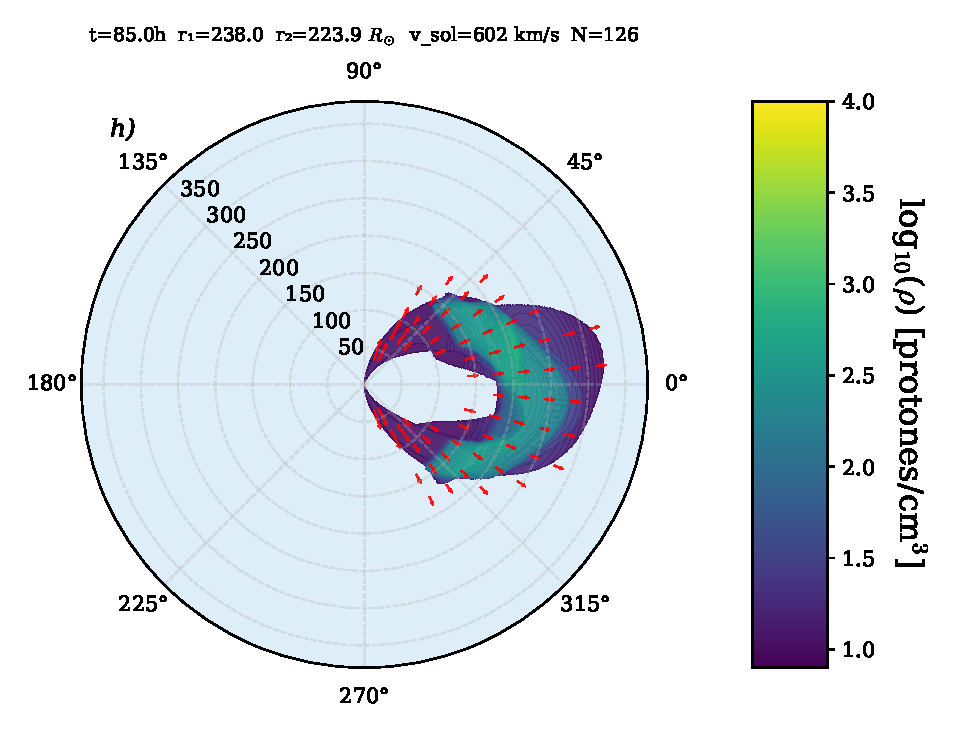
\includegraphics[width=\linewidth]{cme_conjunta_polar_panel8_s1_435_s2_1962.pdf}
        \caption*{(a)}
    \end{subfigure}
    \hfill
    \begin{subfigure}{0.48\linewidth}
        \centering
        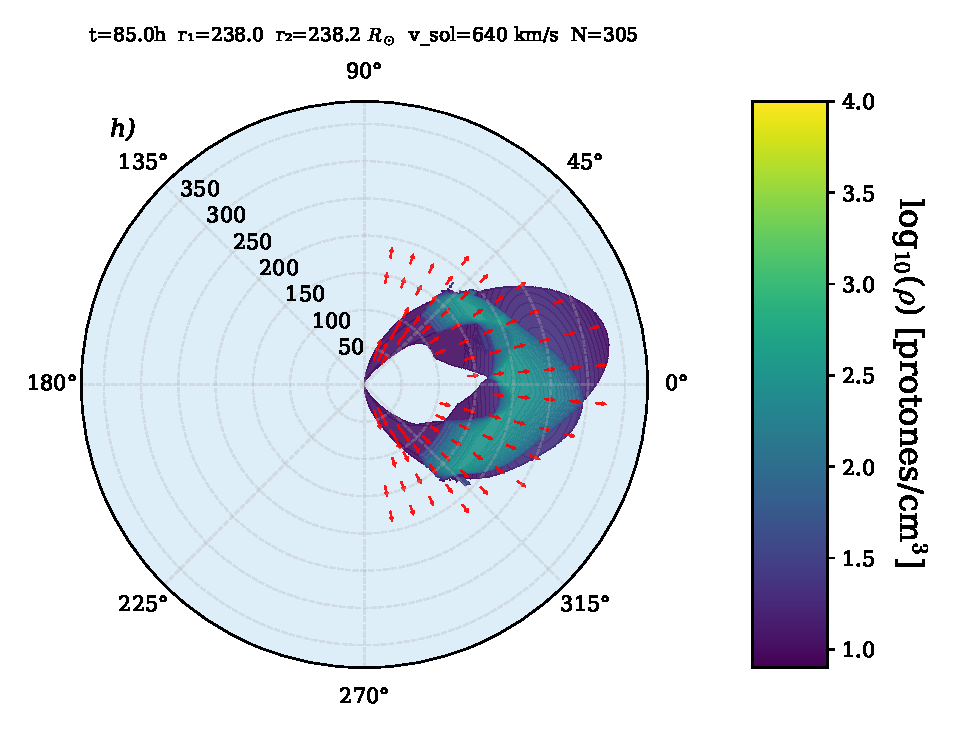
\includegraphics[width=\linewidth]{cme_conjunta_polar_panel8_s1_435_s2_256_2.pdf}
        \caption*{(b)}
    \end{subfigure}
    \caption[Comparación entre paneles finales de la simulación de la interacción de los Casos 1 y 2]{Paneles finales (85 horas) de la simulación de la evolución polar para el Caso 1 (a) y Caso 2 (b). \textit{Nota:} Figura de elaboración propia.}
    \label{fig:CMEsresultantes}
\end{figure}

Siguiendo las series temporales mostradas en las Figuras \ref{Serietiempocaso1} y \ref{Serietiempocaso2}, es posible comparar el comportamiento local de su velocidad y densidad a lo largo de su evolución. En el Caso 1....

En el Caso 2, la serie de tiempo de la densidad en los puntos cercanos al Sol muestran dos picos, lo que indica el paso de las dos CMEs sin interacción; posteriormente, durante la interacción de sus frentes ($\sim 18$ horas), la densidad máxima de cada serie de tiempo describen un comportamiento decreciente para luego aumentar mientras la CME sucesora atraviesa a la precursora ($\sim30$ horas), luego este comportamiento se vuelve lineal con la distancia, puesto que el máximo de cada serie de tiempo --cada distancia al Sol-- disminuye progresivamente; esto debido a una baja diferencia entre las velocidades de las CMEs. Asimismo, la velocidad en puntos cercanos al Sol, presenta dos valles indicando el paso de las dos CMEs con velocidades menores a la del viento solar, en seguida los máximos de cada serie de tiempo describen el comportamiento creciente y posteriormente constante del perfil de velocidad, lo cual coincide con el comportamiento reportado por \text[e.g.,][]{gallagher-2003}, estabilizándose en $\sim640$ km s$^{-1}$. Por consiguiente, la interacción conlleva a una fusión suave entre las CMEs.
